\documentclass[handout, 10pt]{beamer}
%\documentclass[aspectratio=169]{beamer}
\usetheme[background=light,numbering=fraction]{metropolis}           % Use metropolis theme
%\usetheme[background=light]{metropolis}           % Use metropolis theme
\usepackage{appendixnumberbeamer}

\usepackage{tikz}
\usetikzlibrary{fit, arrows.meta, calc}

\usepackage[super,negative]{nth}
\usepackage{url}
\usepackage{amssymb}
\usepackage{amsmath}
\usepackage{mathtools}
\usepackage[labelfont=bf,textfont={it}]{caption}
%\usepackage{subcaption}
%\usepackage[noindentafter]{titlesec}

\usepackage[maxnames=3,maxbibnames=99,mincrossrefs=5,style=trad-abbrv]{biblatex}
\addbibresource{../paper/mprop.bib}
% Make et al.s go all italic
\usepackage{xpatch}
\xpatchbibmacro{name:andothers}{%
	\bibstring{andothers}%
}{%
	\bibstring[\emph]{andothers}%
}{}{}
\DeclareFieldFormat{addendum}{}

\usepackage[binary-units]{siunitx}
\sisetup{range-phrase=--, range-units=single}
%\renewcommand{\deg}{\ensuremath{^{\circ}}\xspace}

\usepackage{microtype}
\usepackage{fontspec}
\usepackage{booktabs}
\usepackage{fontawesome}

\definecolor{graphc1}{RGB}{150,227,240}
\definecolor{graphc2}{RGB}{250,71,37}
\definecolor{graphc3}{RGB}{253,161,77}
\definecolor{graphc4}{RGB}{141,246,135}

% Official colours!

\definecolor{uofguniversityblue}{rgb}{0, 0.219608, 0.396078}

\definecolor{uofgheather}{rgb}{0.356863, 0.32549, 0.490196}
\definecolor{uofgaquamarine}{rgb}{0.603922, 0.72549, 0.678431}
\definecolor{uofgslate}{rgb}{0.309804, 0.34902, 0.380392}
\definecolor{uofgrose}{rgb}{0.823529, 0.470588, 0.709804}
\definecolor{uofgmocha}{rgb}{0.709804, 0.564706, 0.47451}

\definecolor{uofglawn}{rgb}{0.517647, 0.741176, 0}
\definecolor{uofgcobalt}{rgb}{0, 0.615686, 0.92549}
\definecolor{uofgturquoise}{rgb}{0, 0.709804, 0.819608}
\definecolor{uofgsunshine}{rgb}{1.0, 0.862745, 0.211765}
\definecolor{uofgpumpkin}{rgb}{1.0, 0.72549, 0.282353}
\definecolor{uofgthistle}{rgb}{0.584314, 0.070588, 0.447059}
\definecolor{uofgpillarbox}{rgb}{0.701961, 0.047059, 0}
\definecolor{uofglavendar}{rgb}{0.356863, 0.301961, 0.580392}

\definecolor{uofgsandstone}{rgb}{0.321569, 0.278431, 0.231373}
\definecolor{uofgforest}{rgb}{0, 0.317647, 0.2}
\definecolor{uofgburgundy}{rgb}{0.490196, 0.133333, 0.223529}
\definecolor{uofgrust}{rgb}{0.603922, 0.227451, 0.023529}

\newcommand{\lesspreceq}[1]{\prescript{}{#1}{\preceq}\ }

\title{Graph Models and Maximum Common Subgraph for Character Analysis}
\date{\nth{18} April, 2017}
\author{
	Kyle A. Simpson (2029567s) \\
	\tiny{\faGithub{} \url{https://github.com/FelixMcFelix} \hspace{0.5em} \faGlobe{} \url{https://mcfelix.me}}
}
\institute{University of Glasgow}

\begin{document}
\maketitle

%\begin{frame}{Table of contents}
%	\setbeamertemplate{section in toc}[sections numbered]
%	\tableofcontents[hideallsubsections]
%\end{frame}

\section{The Problem}

\begin{frame}{Modern Computer Vision Models}
%	\only<1|handout:1>{%
		For modern computer vision tasks, machine learning models and vector-space representations dominate.
		Typically these capture high-dimensional keypoints, consider low-level codings and/or learn data features through statistical inference.
		These are powerful approaches with proven effectiveness.
		
		\pause
		
		\begin{alertblock}{But...}
			\begin{itemize}[<+(1)- | alert@+(1)>]
				\item Popular representations are high-dimension vectors of real values---it can be hard to intuit their meaning!
				\begin{itemize}
					\item We can't look at e.g., a convolution kernel, and see what transformation it represents.
				\end{itemize}
				\item How can we then reason about a dependent system's robustness? Sensitive to odd phenomena; can be exploited by \emph{adversarial images} \cite{AdversarialML}.
			\end{itemize}
		\end{alertblock}
%	}%
\end{frame}

\begin{frame}{Why Graph Models?}
	\begin{columns}
		\begin{column}{0.6\linewidth}
			Graph models decompose problems into \alert{elements} and their \alert{relationships}---a sensible encoding for many domains.
			We can benefit greatly if they can be used sensibly within computer vision:
			
			\begin{itemize}[<+(1)- | alert@+(1)>]
				\item More intuitive problem models.
				\begin{itemize}
					\item We can manually assess whether a representation matches image content, and correct if need be.
				\end{itemize}
				\item Easier to assess model robustness.
				\item We can use standard, well-understood graph search and similarity algorithms, \emph{independent of domain}!
			\end{itemize}
		\end{column}
	
		\begin{column}{0.4\linewidth}
			\begin{figure}
			\centering
			\resizebox{\linewidth}{!}{
				\huge
				\begin{tikzpicture}
				\node[inner sep=5pt] (sagrada1) at (0,0)
				{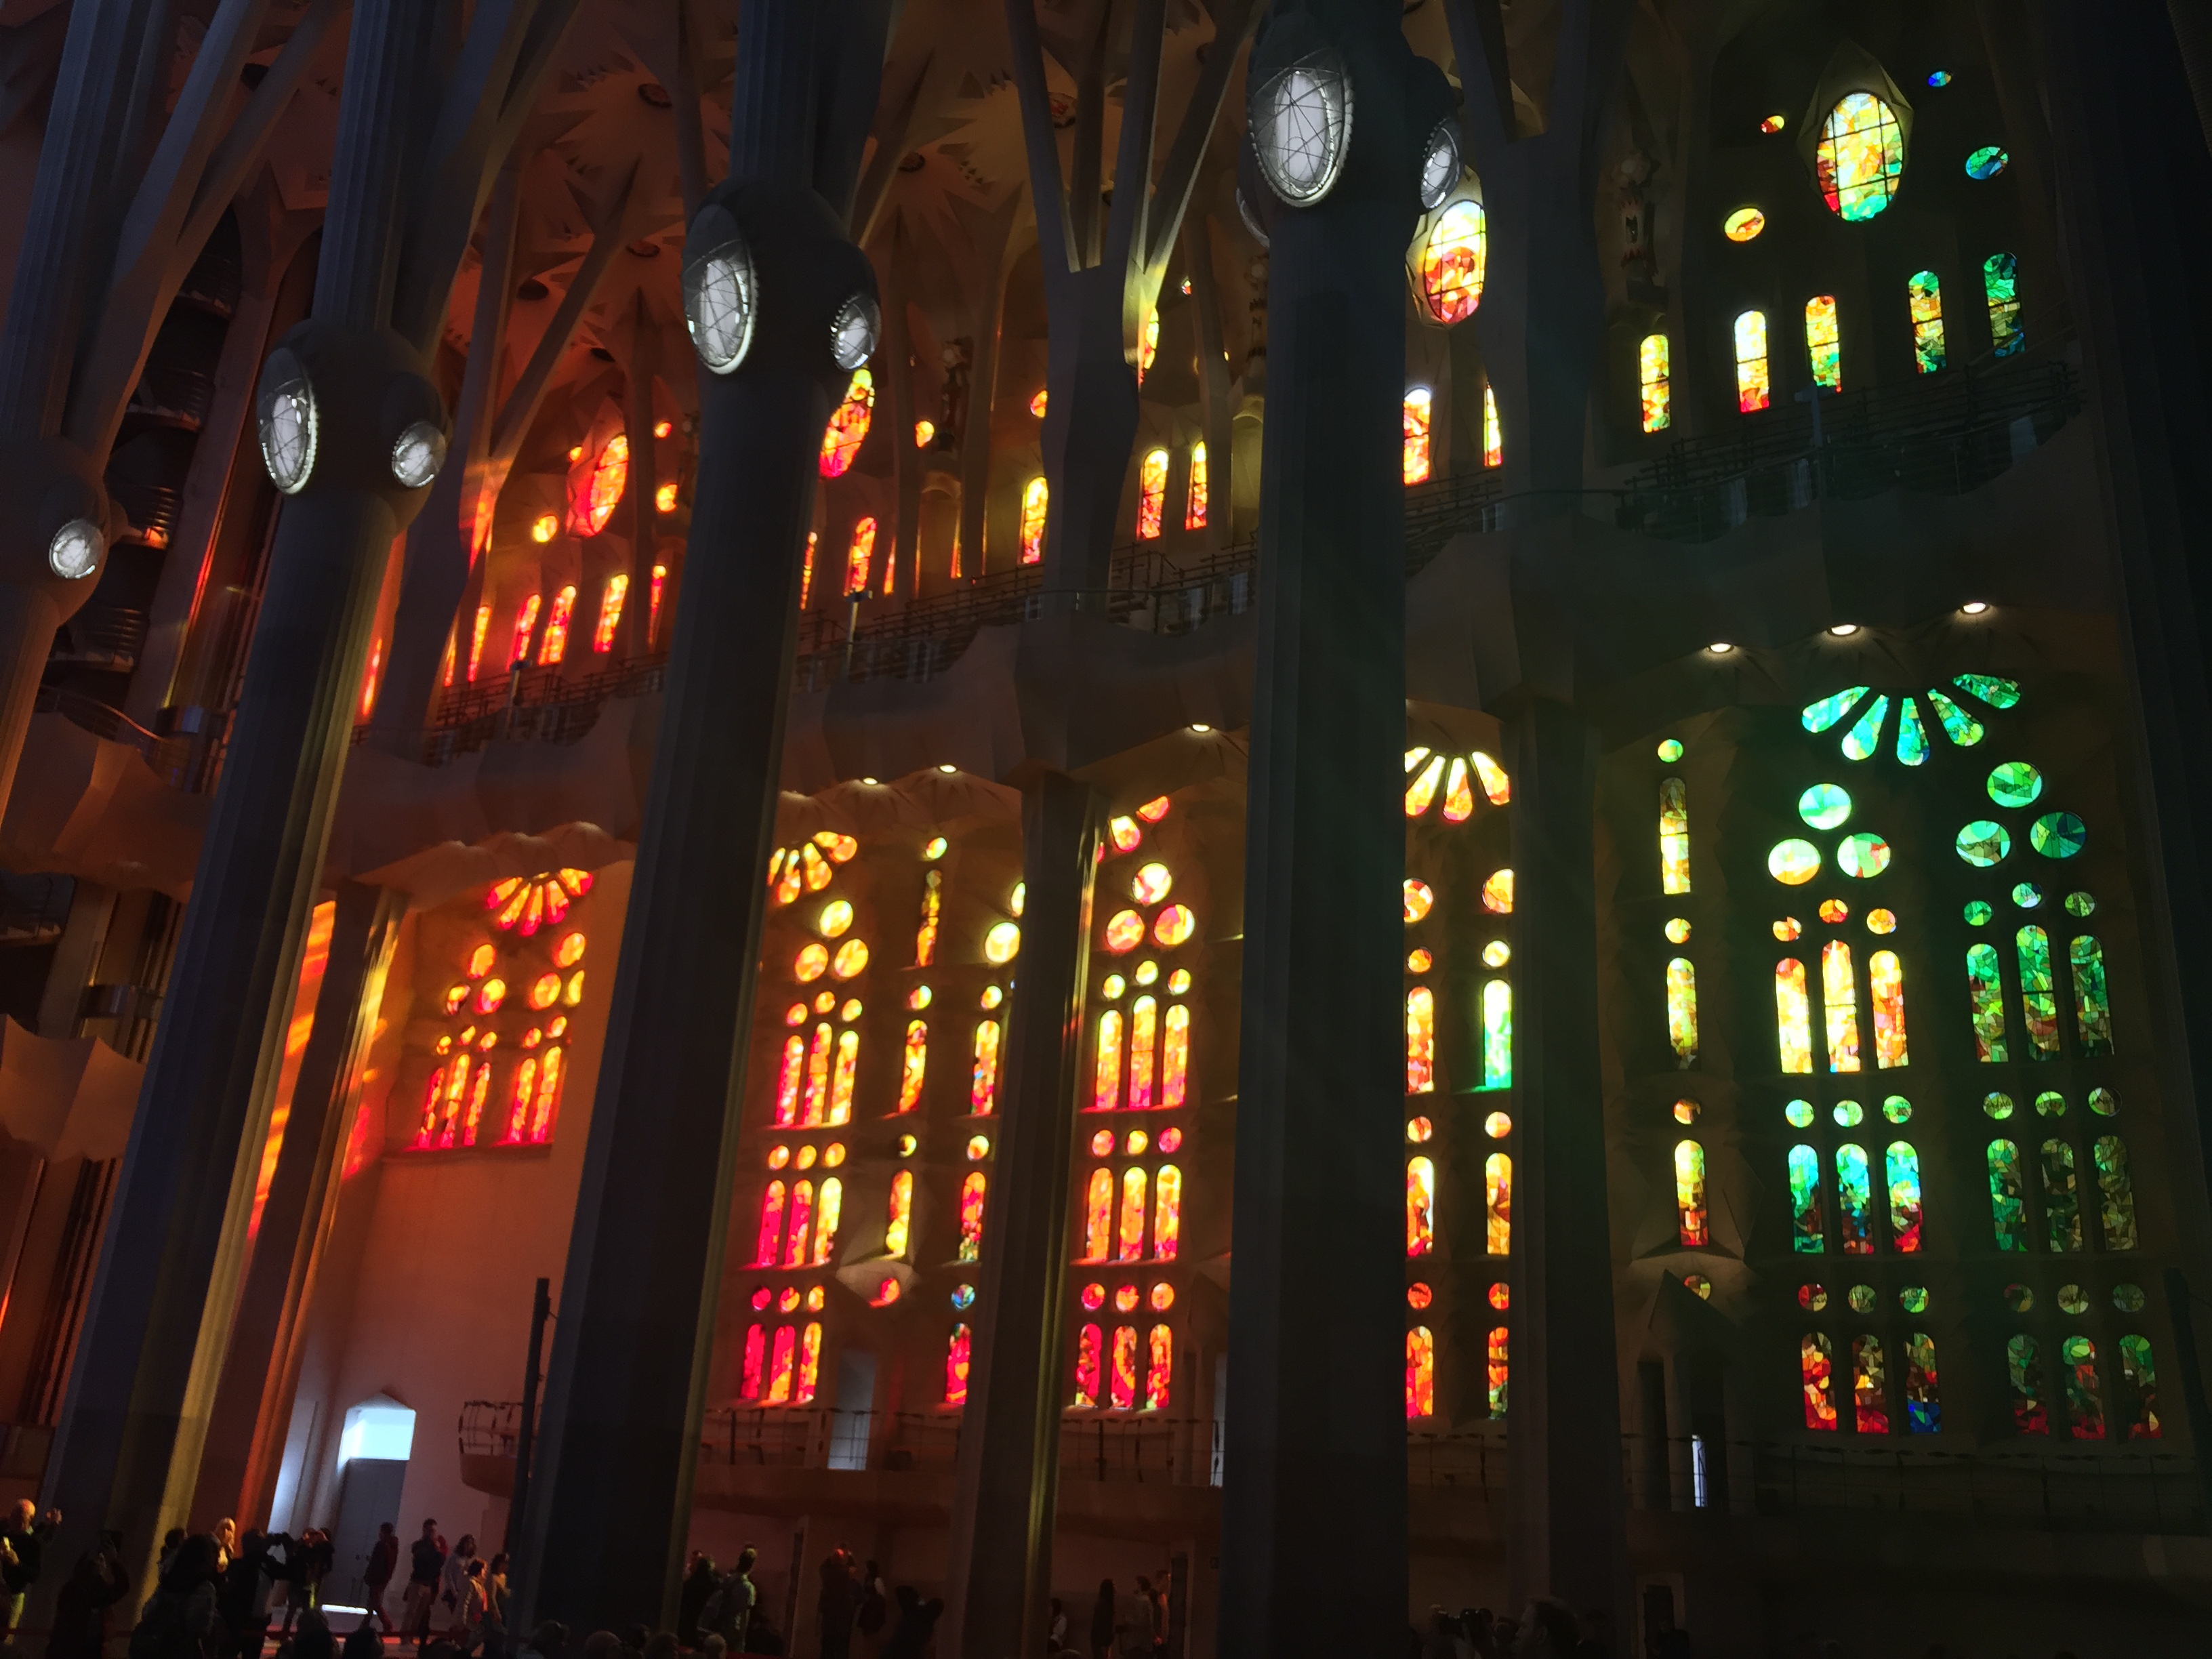
\includegraphics[width=0.9\linewidth]{../paper/images/IMG_3267.JPG}};
				\node[inner sep=5pt] (sagrada2) at (10,0)
				{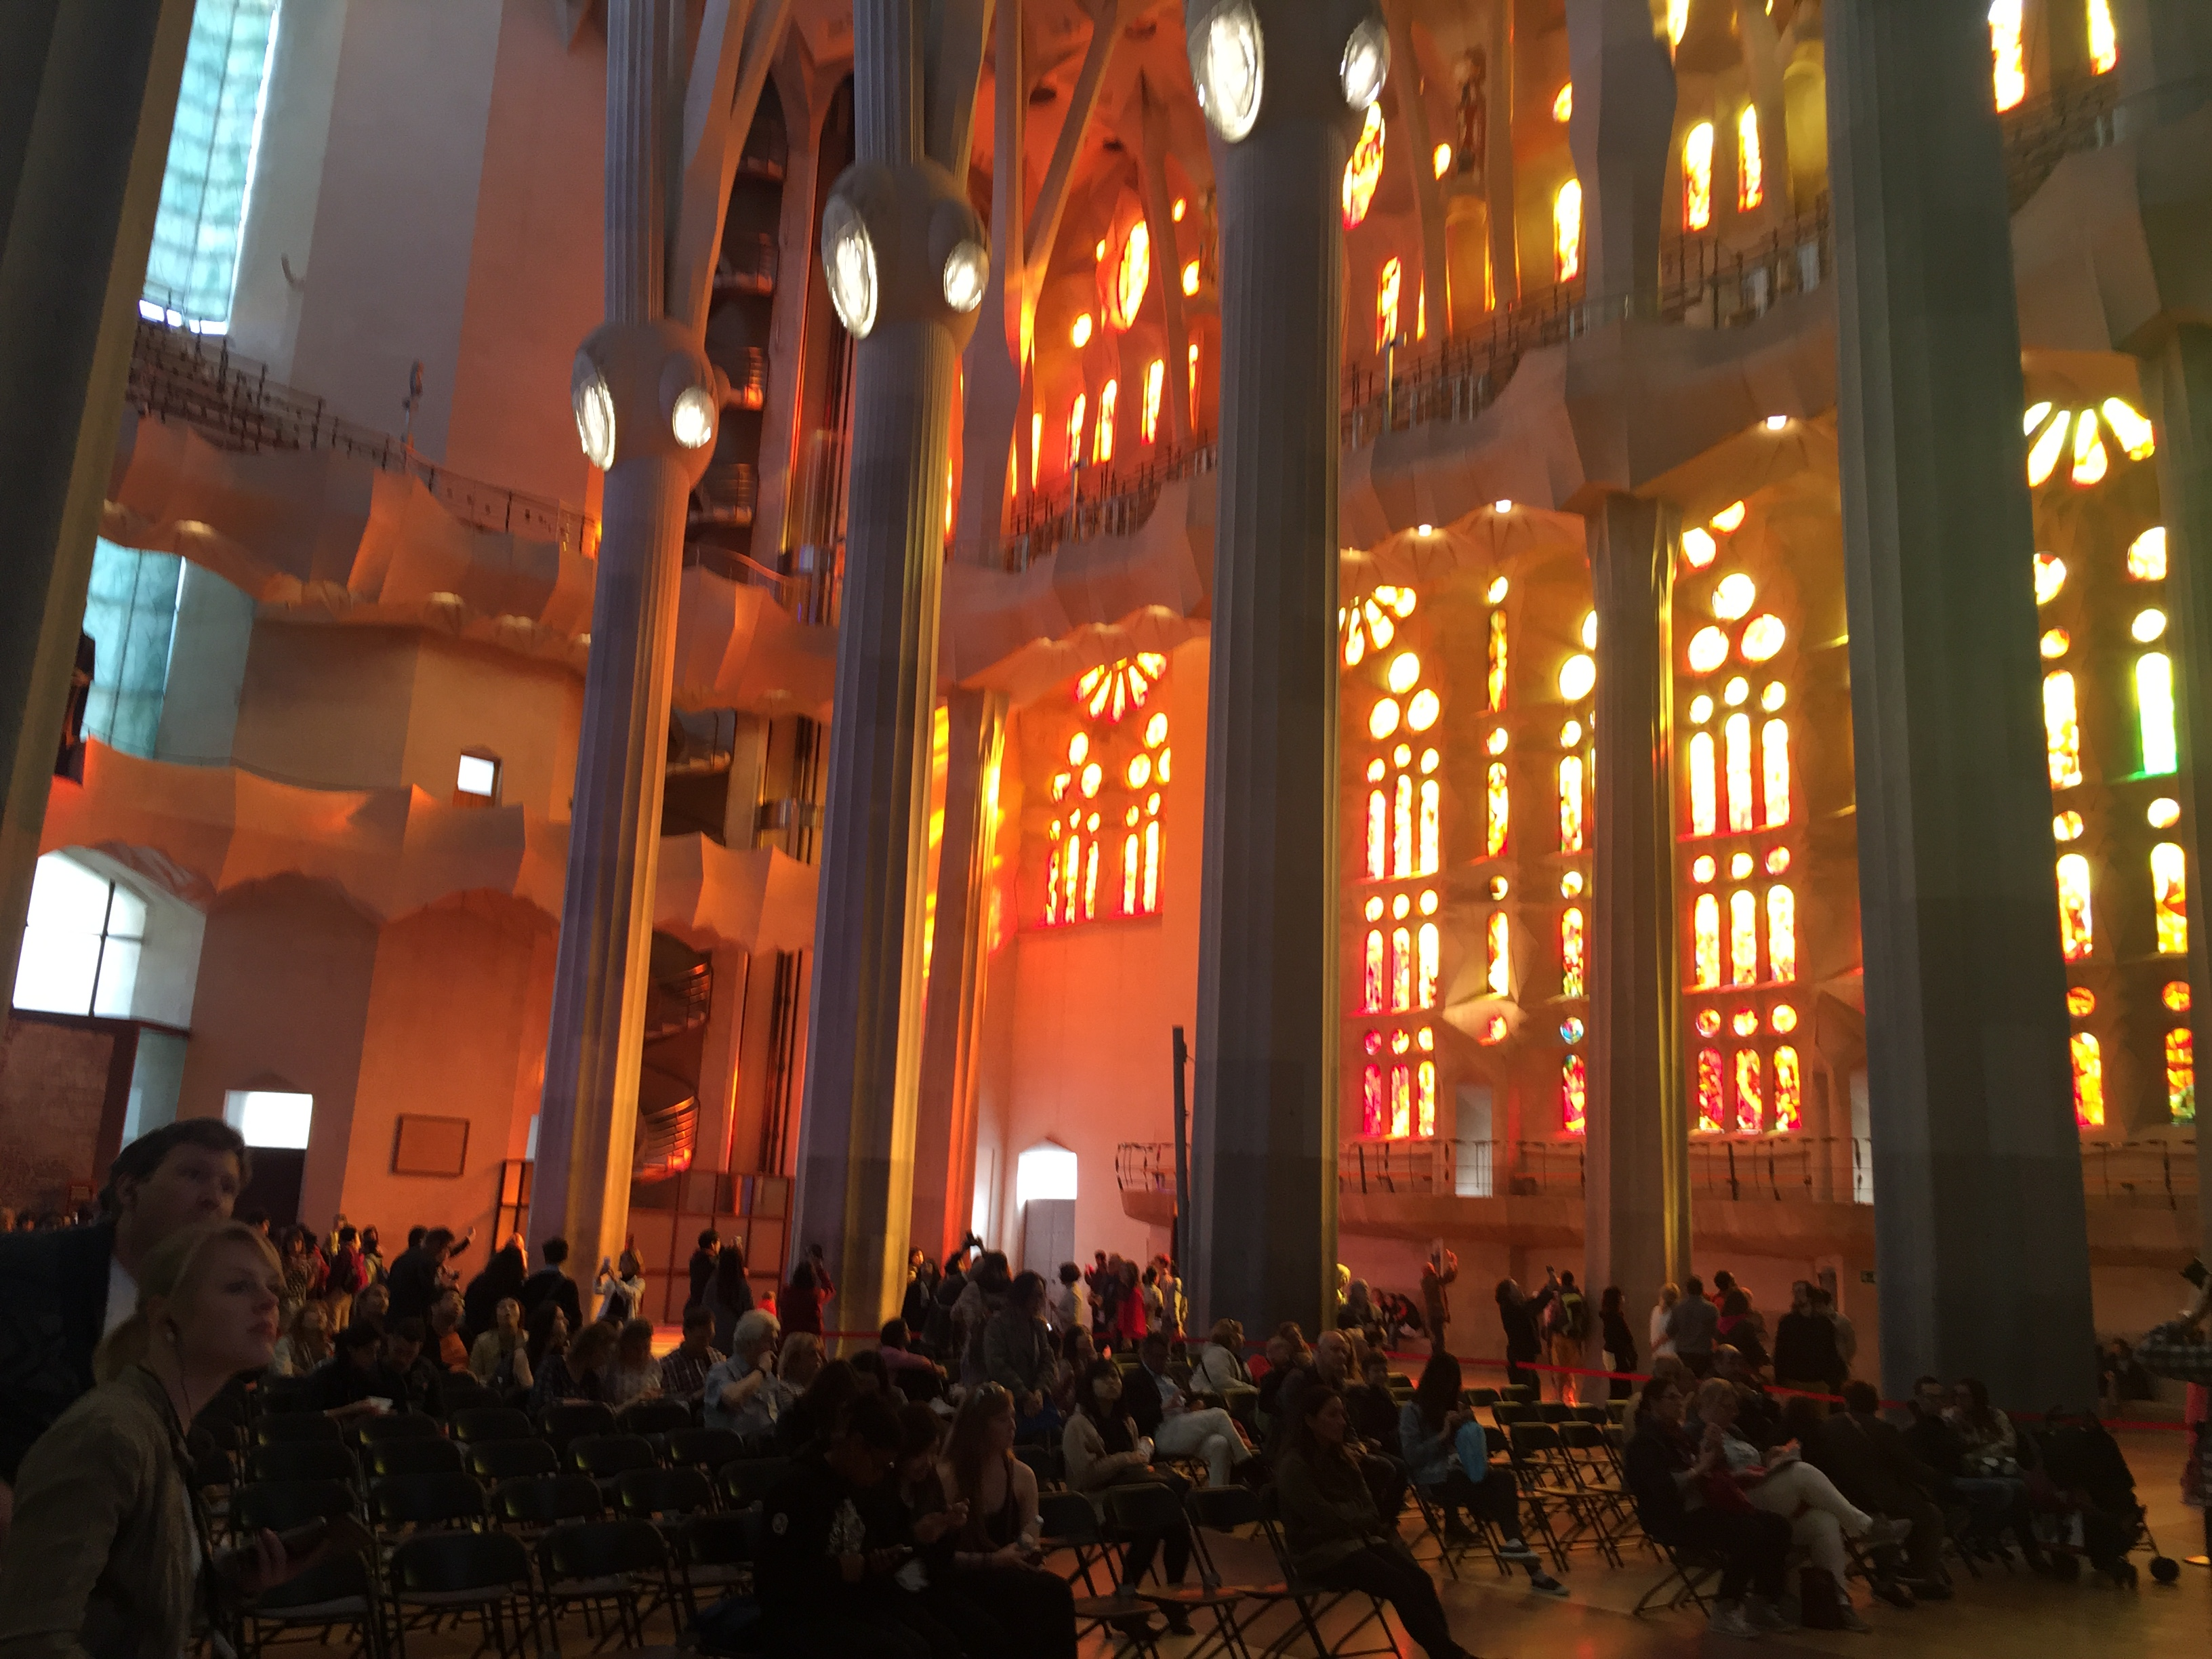
\includegraphics[width=0.9\linewidth]{../paper/images/IMG_3268.JPG}};
				
				\node[inner sep=5pt] (graph1) at (0,-6)
				{
					\begin{tikzpicture}
					\node[draw, circle, fill=graphc2] (n1) at (0,-1) {};
					\node[draw, circle, fill=graphc3] (n2) at (1,-0.67) {};
					\node[draw, circle, fill=graphc4] (n3) at (2,-0.33) {};
					\node[draw, circle, fill=graphc2] (n4) at (0,-2) {};
					\node[draw, circle, fill=graphc3] (n5) at (1,-1.9) {};
					\node[draw, circle, fill=graphc4] (n6) at (2,-1.8) {};
					
					\draw[<->] (n1) -- (n2);
					\draw[<->] (n2) -- (n3);
					\draw[<->] (n1) -- (n4);
					\draw[<->] (n2) -- (n5);
					\draw[<->] (n4) -- (n5);
					\draw[<->] (n5) -- (n6);
					\end{tikzpicture}
				};
				
				\node[inner sep=5pt] (graph2) at (10,-6)
				{
					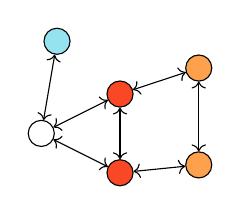
\begin{tikzpicture}
					\node[draw, circle] (n0) at (-1,-1.5) {};
					\node[draw, circle, fill=graphc1] (n7) at (-0.8,-0.33) {};
					\node[draw, circle, fill=graphc2] (n1) at (0,-1) {};
					\node[draw, circle, fill=graphc3] (n2) at (1,-0.67) {};
					\node[draw, circle, fill=graphc2] (n4) at (0,-2) {};
					\node[draw, circle, fill=graphc3] (n5) at (1,-1.9) {};
					
					\draw[<->] (n0) -- (n1);
					\draw[<->] (n0) -- (n4);
					\draw[<->] (n0) -- (n7);
					\draw[<->] (n1) -- (n2);
					\draw[<->] (n1) -- (n4);
					\draw[<->] (n2) -- (n5);
					\draw[<->] (n4) -- (n5);
					\end{tikzpicture}
				};
				
				\draw[->,thick] (sagrada1.east) -- (sagrada2.west)
				node[midway,fill=bg] {Similarity};
				\draw[->,thick] (graph1.east) -- (graph2.west)
				node[midway,fill=bg] {Similarity};
				
				\draw[->,thick] (sagrada1.south) -- (graph1.north)
				node[midway,fill=bg] {Transform};
				\draw[->,thick] (sagrada2.south) -- (graph2.north)
				node[midway,fill=bg] {Transform};
			\end{tikzpicture}}
			
			\caption{The core hypothesis---can we translate image similarity to graph similarity?}
			\end{figure}
		\end{column}
	\end{columns}
\end{frame}

\begin{frame}{Core Questions}
\begin{itemize}[<+- | alert@+>]
	\item Are current graph models for generic image content suitable and/or effective?
	\item How useful is exact similarity (i.e.\ Maximum Common Subgraph) on new algorithms for simpler domain models?
	\begin{itemize}
		\item I.e. character recognition, word spotting.
	\end{itemize}
	\item How does this combination fare against existing graph models and similarity metrics in that domain?
\end{itemize}
\end{frame}

\section{Graph Similarity}

\begin{frame}{Quick Preliminaries}
	Given a graph $\mathcal{G}=(V,E)$, with vertex set $V$ and edge set $E$:
	
	\begin{itemize}
		\item $\text{Ord}(\mathcal{G}) = |V|$, the vertex count or \emph{order} of $\mathcal{G}$
		\item $\text{Sz}(\mathcal{G}) = |E|$, the edge count or \emph{size} of $\mathcal{G}$
	\end{itemize}
\end{frame}

\begin{frame}{Subgraph Isomorphism: Graph Search}

\begin{columns}
\begin{column}{0.4\linewidth}
\begin{figure}
	\resizebox{\linewidth}{!}{\begin{tikzpicture}
	
	\node[label=below:{$\mathcal{P}$}] (p) at (0,0){
		\begin{tikzpicture}[scale=1]
		\begin{scope}[auto, every node/.style={draw,circle,minimum size=2em,inner sep=1},node distance=2cm]
		\node[draw, circle] (n1) at (0,0) {a};
		\node[draw, circle] (n2) at (0,-1) {c};
		\node[draw, circle] (n3) at (1,0) {b};
		\node[draw, circle] (n4) at (1,-1) {d};
		\end{scope}
		
		\draw[-] (n1) -- (n3);
		\draw[-] (n2) -- (n4);
		\draw[-] (n1) -- (n4);
		\draw[-] (n2) -- (n3);
		\draw[-] (n3) -- (n4);
		\end{tikzpicture}
	};
	
	\node[label=below:{$\mathcal{T}$}] (t) at (4,0){
		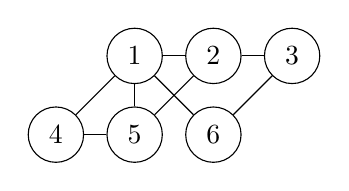
\begin{tikzpicture}[scale=1]
		\begin{scope}[auto, every node/.style={draw,circle,minimum size=2em,inner sep=1},node distance=2cm]
		\node[draw, circle] (n1) at (2,0) {2};
		\node[draw, circle] (n2) at (0,-1) {4};
		\node[draw, circle] (n3) at (1,0) {1};
		\node[draw, circle] (n4) at (1,-1) {5};
		
		\node[draw, circle] (n5) at (2,-1) {6};
		\node[draw, circle] (n6) at (3,0) {3};
		\end{scope}
		
		\draw[-] (n1) -- (n3);
		\draw[-] (n2) -- (n4);
		\draw[-] (n1) -- (n4);
		\draw[-] (n2) -- (n3);
		\draw[-] (n3) -- (n4);
		
		\draw[-] (n5) -- (n6);
		\draw[-] (n1) -- (n6);
		\draw[-] (n3) -- (n5);
		\end{tikzpicture}
	};
	
	\node[label=below:{Embedding}] (em) at (2,-3){
		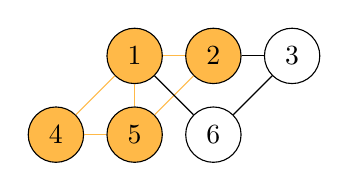
\begin{tikzpicture}[scale=1]
		\begin{scope}[auto, every node/.style={draw,circle,minimum size=2em,inner sep=1},node distance=2cm]
		\node[draw, circle, fill=uofgpumpkin] (n1) at (2,0) {2};
		\node[draw, circle, fill=uofgpumpkin] (n2) at (0,-1) {4};
		\node[draw, circle, fill=uofgpumpkin] (n3) at (1,0) {1};
		\node[draw, circle, fill=uofgpumpkin] (n4) at (1,-1) {5};
		
		\node[draw, circle] (n5) at (2,-1) {6};
		\node[draw, circle] (n6) at (3,0) {3};
		\end{scope}
		
		\draw[-, color=uofgpumpkin] (n1) -- (n3);
		\draw[-, color=uofgpumpkin] (n2) -- (n4);
		\draw[-, color=uofgpumpkin] (n1) -- (n4);
		\draw[-, color=uofgpumpkin] (n2) -- (n3);
		\draw[-, color=uofgpumpkin] (n3) -- (n4);
		
		\draw[-] (n5) -- (n6);
		\draw[-] (n1) -- (n6);
		\draw[-] (n3) -- (n5);
		\end{tikzpicture}
	};
	
	\draw[->, thick] ($(em.north) + (0,1)$) -- (em.north);
	
	\end{tikzpicture}}

\caption{Example of SIP---$\mathcal{P}$'s embedding in $\mathcal{T}$ is shown in orange.}
\end{figure}
\end{column}

\begin{column}{0.6\linewidth}
	The \alert{subgraph isomorphism problem} (SIP): given a pattern graph $\mathcal{P}$ and a target graph $\mathcal{T}$, can we find a reproduction of $\mathcal{P}$ in $\mathcal{T}$?
	
	\begin{itemize}
		\item Non-induced? Preserves only adjacency. Can delete edges of $\mathcal{T}$ for embedding.
		\item Induced? Preserves both adjacency and non-adjacency---stricter matching!
		\item Feasible for graphs of order $10^3$.
	\end{itemize}

	I.e. can we find the image graph of a road sign inside a photograph?
\end{column}

\end{columns}
\end{frame}

\begin{frame}{Maximum Common Subgraph: Graph Similarity}
\begin{columns}
	\begin{column}{0.65\linewidth}
		The \alert{maximum common subgraph problem} (MCS): given a pattern graph $\mathcal{P}$ and a target graph $\mathcal{T}$, what is the largest subgraph of $\mathcal{P}$ reproduced in $\mathcal{T}$?
		
		\begin{itemize}
			\item Induced and non-induced variants, as before.
			\item Feasible for graphs of order... 30--40.
			\item We now have a rough similarity metric: $\text{Ord}(\text{MCS}(\mathcal{P}, \mathcal{T}))$.
		\end{itemize}
		
		I.e. can we find the image graph of a road sign inside a photograph, where it is slightly obscured? (\emph{Occlusion invariant matching}).
	\end{column}
	\begin{column}{0.35\linewidth}
		\begin{figure}
		\resizebox{\columnwidth}{!}{
			\begin{tikzpicture}
			
			\node[label=below:{$\mathcal{P}$}] (p) at (0,0){
				\begin{tikzpicture}[scale=1]
				\begin{scope}[auto, every node/.style={minimum size=2em,inner sep=1},node distance=2cm]
				\node[draw, circle] (n1) at (0,0) {a};
				\node[draw, circle] (n2) at (0,-1) {c};
				\node[draw, circle] (n3) at (1,0) {b};
				\node[draw, circle] (n4) at (1,-1) {d};
				
				\draw[-] (n1) -- (n3);
				\draw[-] (n2) -- (n4);
				\draw[-] (n1) -- (n4);
				\draw[-] (n2) -- (n3);
				\draw[-] (n3) -- (n4);
				\end{scope}
				\end{tikzpicture}
			};
			
			\node[label=below:{$\mathcal{T}$}] (t) at (3,0){
				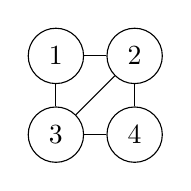
\begin{tikzpicture}[scale=1]
				\begin{scope}[auto, every node/.style={draw,circle,minimum size=2em,inner sep=1},node distance=2cm]
				\node[draw, circle] (n1) at (0,0) {1};
				\node[draw, circle] (n2) at (0,-1) {3};
				\node[draw, circle] (n3) at (1,0) {2};
				\node[draw, circle] (n4) at (1,-1) {4};
				\end{scope}
				
				\draw[-] (n1) -- (n3);
				\draw[-] (n2) -- (n4);
				\draw[-] (n1) -- (n2);
				\draw[-] (n2) -- (n3);
				\draw[-] (n3) -- (n4);
				
				\end{tikzpicture}
			};
			
			\node[label=below:{Embedding}] (em) at (1.5,-3){
				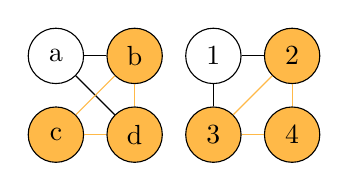
\begin{tikzpicture}[scale=1]
				\begin{scope}[auto, every node/.style={draw,circle,minimum size=2em,inner sep=1},node distance=2cm]
				\node[draw, circle] (n1) at (0,0) {a};
				\node[draw, circle, fill=uofgpumpkin] (n2) at (0,-1) {c};
				\node[draw, circle, fill=uofgpumpkin] (n3) at (1,0) {b};
				\node[draw, circle, fill=uofgpumpkin] (n4) at (1,-1) {d};
				
				\draw[-] (n1) -- (n3);
				\draw[-, color=uofgpumpkin] (n2) -- (n4);
				\draw[-] (n1) -- (n4);
				\draw[-, color=uofgpumpkin] (n2) -- (n3);
				\draw[-, color=uofgpumpkin] (n3) -- (n4);
				
				\node[draw, circle] (n1') at (2,0) {1};
				\node[draw, circle, fill=uofgpumpkin] (n2') at (2,-1) {3};
				\node[draw, circle, fill=uofgpumpkin] (n3') at (3,0) {2};
				\node[draw, circle, fill=uofgpumpkin] (n4') at (3,-1) {4};
				
				
				\draw[-] (n1') -- (n3');
				\draw[-, color=uofgpumpkin] (n2') -- (n4');
				\draw[-] (n1') -- (n2');
				\draw[-, color=uofgpumpkin] (n2') -- (n3');
				\draw[-, color=uofgpumpkin] (n3') -- (n4');
				\end{scope}
				\end{tikzpicture}
			};
			
			\draw[->, thick] ($(em.north) + (0,1)$) -- (em.north);
			
		\end{tikzpicture}}
		
		\caption{Example of MCS. The result's embedding in both $\mathcal{P}$ and $\mathcal{T}$ is shown in orange.}
		\end{figure}
	\end{column}
\end{columns}
\end{frame}

\begin{frame}{Graph Edit Distance: Graph Dissimilarity}
	We can count the number of vertex additions and deletions needed to transform $\mathcal{P}$ into $\mathcal{T}$---the \alert{graph edit distance} (GED).
	
	$$ \text{GED}(\mathcal{P}, \mathcal{T}) = \text{Ord}(\mathcal{P}) + \text{Ord}(\mathcal{T}) - 2 \times \text{Ord}(\text{MCS}(\mathcal{P}, \mathcal{T})) $$
	
	This is the core metric used in this work---note that this gives edge changes zero cost.
\end{frame}

\section{State-of-the-art Generic Models}

\begin{frame}{State-of-the-art Generic Models}
\begin{itemize}
	\item Present work (such as \citeauthor{Plane-Graphs-From-Images} \cite{Plane-Graphs-From-Images} or \citeauthor{Submap-Iso-Images} \cite{Submap-Iso-Images}) focuses on building plane graphs for their algorithmic properties.
	\begin{itemize}
		\item They extract interest pixel locations then compute the \alert{Delaunay triangulation} \cite{Delaunay}, building a triangle mesh s.t.\ no point falls inside any triangle's circumcircle.
	\end{itemize}
	
	\item \citeauthor{Plane-Graphs-From-Images} attempt to extend this with structural cues from image segmentation.
	
	\item These don't appear to capture any discriminative features: these works focus on matching elements \emph{within} an image, and \textbf{not between images}. Is this the case?
\end{itemize}
\end{frame}

\begin{frame}{Putting \citeauthor{Plane-Graphs-From-Images} to the Test}
\begin{columns}
	\begin{column}{0.8\linewidth}
		I reimplemented their work, with two experiments in mind using the \alert{$k\downarrow$} MCS algorithm \cite{Between-MCS-SIP}:
		
		\begin{enumerate}
			\item Is the graph of a test image from the Berkeley Segmentation Dataset rotated $180^{\circ}$ isomorphic to itself? I.e. is this transformation isotropic?
			
			\item How similar are two adjacent frames from Sergio Leone's \emph{The Good, the Bad and the Ugly}?
		\end{enumerate}
	
		For this, I augment graphs with positional data, applying euclidean distance filtering to help matching along.
	%	In the first case, perfect segmentation information is known.
	%	In the second, this must be done algorithmically.
	\end{column}

	\begin{column}{0.2\linewidth}
		\begin{figure}
			\centering
			\begin{figure}
				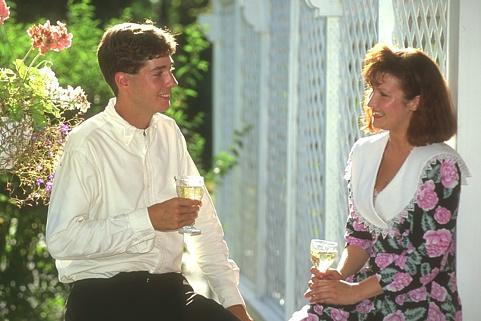
\includegraphics[width=\linewidth]{../paper/images/bsd-157055}
				
	%			\caption{BSD test image}
	%			\label{fig:explor-bsd}
	%		\end{figure}
	%		~
	%		\begin{figure}
				
\includegraphics[width=\linewidth]{../paper/images/gbu2}
				
	%			\caption{Film frame 1}
	%			\label{fig:explor-ff1}
	%		\end{figure}
	%		~
	%		\begin{figure}
				
\includegraphics[width=\textwidth]{../paper/images/gbu3}
				
	%			\caption{Film frame 2}
	%			\label{fig:explor-ff2}
			\caption{Three test images: BSD, GBU1 and GBU2.}
			\end{figure}
		\end{figure}
	\end{column}
\end{columns}
\end{frame}

\begin{frame}{The Results?}
\begin{columns}
	\begin{column}{0.4\linewidth}
		\begin{table}[h]
			\centering
			\resizebox{0.7\linewidth}{!}{
				\begin{tabular}{lSS}
					\toprule
					\multicolumn{1}{c}{Image} & \multicolumn{1}{c}{Order} & \multicolumn{1}{c}{Size} \\ \midrule
					BSD & \num{245} & \num{707} \\
					BSD-180 & \num{247} & \num{705} \\
					GBU1 & \num{264} & \num{755} \\
					GBU2 & \num{260} & \num{743} \\
					\bottomrule
				\end{tabular}
			}
			
			\caption{
				Graph stats for real-world images.
			}
		\end{table}
		\begin{table}[h]
			\centering
			\resizebox{\linewidth}{!}{
			\begin{tabular}{cccc}
				\toprule
				Experiment & Except-$k$ & $\text{Ord}(\mathit{MCS})$ & Overlap (\si{\percent}) \\ \midrule
				1 & $[61, 111]$ & $[134, 184]$ & 54.6--72.2 \\
				2 & $[38, 217]$ & $[47, 226]$ & 18.1--86.9 \\
				\bottomrule
			\end{tabular}
			}
			
			\caption{
				Observed similarity bounds between real-world images.
				\label{tab:badgraphs}
			}
		\end{table}
	\end{column}

	\begin{column}{0.6\linewidth}
		Findings (after 5 days running on fatanode-01):
		\begin{itemize}
			\item Negative results on both counts!
			\begin{itemize}
				\item \alert{No isomorphism in first experiment}, with lower similarity than expected.
				\item Wide bound in second experiment---\alert{uniform graph structure hinders matching performance}.
			\end{itemize}
			\item Not isotropic---inherits sensitivities from interest pixel detector.
			\item Depends heavily on perfect segmentation, to detriment of matching.
		\end{itemize}
	\end{column}
\end{columns}
\end{frame}

\frame[standout]{
	These are high-order, high-size graphs with uniform structure and no discriminative features.
	This approach is \emph{not} appropriate for real-world matching!
}

\section{The Conclusion?}

\begin{frame}[standout]
Conclusion!
\end{frame}

\begin{frame}{Conclusion}
	\begin{itemize}[<+- | alert@+>]
		\item One thing
		\item Two thing
		\item Red Thing
		\item Blue thing
	\end{itemize}

	\alert{\textbf{Any questions?}}
\end{frame}

\appendix

\begin{frame}[allowframebreaks]{References}

\printbibliography[heading=none]

\end{frame}

\end{document}